\documentclass[conference]{IEEEtran}
\usepackage[utf8]{inputenc}
\usepackage{amsmath,amssymb,amsthm}
\usepackage{graphicx}
\usepackage{booktabs}
\usepackage{algorithm}
\usepackage{algpseudocode}
\usepackage[hidelinks]{hyperref}

\newtheorem{theorem}{Theorem}
\newcommand{\cset}{\Gamma}

\begin{document}

\title{Conformal Routing for Token-Efficient Object Retrieval over a Persistent Semantic Map}

\author{
\IEEEauthorblockN{Fernando Hernández Cantú (A00841856)
Luis Álvaro Rosales Salazar (A01255674)\\
Alfonso José Morales Mallozzi (A00841550)
Verónica Paola Zapata Sánchez (A01199193)}
\IEEEauthorblockA{TC2038 Analysis and Design of Advanced Algorithms\\
Tecnológico de Monterrey}
}

\maketitle

\begin{abstract}
A household robot must turn commands such as ``bring me the red can from the kitchen'' into one object of a
persistent scene graph. Serializing the graph into an LLM prompt costs tokens linear in the number of objects;
CLIP retrieval is cheap but fails on abstract and negated requests. We let the LLM only parse the command,
resolve location by geometry, rank objects with fused CLIP image and name scores, and build a split-conformal
candidate set whose size routes the command: small sets are answered by CLIP, large ones are verified by a
vision-language model (VLM) over a numbered crop grid. On 114 held-out commands (5 repeats, temperature 0),
the router reaches 81.4\% accuracy against 70.2\% for the full-graph prompt and 78.1\% for CLIP alone, keeps
LLM tokens constant in graph size, holds the conformal coverage guarantee, and degrades least under 25\% label noise.
\end{abstract}

\section{Part I: Algorithmic Analysis}

\subsection{Q1. Problem Definition, Motivation and Assumptions}
\textbf{Input.} A scene graph $G=(R\cup H\cup O, E)$ of rooms $R$ (polygons), surfaces $H$ (furniture poses)
and objects $O$, with edges $\mathrm{contains}(r,h)$ and $\mathrm{on}(h,o)$. Each $o\in O$ has a detector
label $\ell_o$, a CLIP image embedding $e_o\in\mathbb{S}^{d-1}$ ($d=512$), a position $p_o\in\mathbb{R}^3$ and a crop
$I_o$. A command $t$ in English or Spanish. A calibration set $\mathcal{D}=\{(t_i,Y_i)\}_{i=1}^n$ of commands with
their sets of right objects $Y_i\subseteq O$.

\textbf{Output.} One object $\hat o\in O$, a question over a candidate set $\cset\subseteq O$, or ``not found''.

\textbf{Objective.} Maximize $P(\hat o\in Y)$ subject to (i) a model-token budget per command,
(ii) marginal coverage $P(Y\cap\cset\neq\emptyset)\ge 1-\alpha$ of the candidate set, and (iii) a VLM call rate
set by the operator. The unoptimized reference serializes all of $O$ into the prompt, costing $\Theta(|O|)$ tokens.

\textbf{Computational model.} One 8\,GB GPU (RTX 4060 Laptop; the robot target is a Jetson Orin) serving one
model at a time through Ollama: a parser LLM (Qwen3-8B), a VLM (Qwen2.5-VL-7B~\cite{bai2025qwen25vl}) and CLIP
ViT-B/32~\cite{radford2021clip}. Model calls dominate cost; vector and geometric work is sub-millisecond to
milliseconds.

\textbf{Assumptions.} The map layout is known (RoboCup@Home arena); the scene is static during a command;
calibration and test commands are exchangeable; embeddings are $\ell_2$-normalized; labels may be wrong.

\textbf{Why this approach.} Scene-graph systems either let an LLM read the graph
(SayPlan~\cite{rana2023sayplan}, ConceptGraphs~\cite{gu2024conceptgraphs}) or retrieve by CLIP
similarity (HOV-SG~\cite{werby2024hovsg}). The first scales with $|O|$, the second fails on abstract queries.
Conformal prediction~\cite{vovk2005algorithmic,angelopoulos2023gentle} turns CLIP scores into sets with a
distribution-free guarantee, and KnowNo~\cite{ren2023knowno} showed that set size is a usable signal for when
a robot should seek help; we use it to decide when to pay for a VLM.

\subsection{Q2. Core Algorithm and Correctness}
The parser returns $(\tau,a,\rho,r)$: target, anchor, relation (\emph{on}/\emph{next to}) and room, under a JSON
schema enforced by constrained decoding. Geometry filters $O$ to the room polygon and to objects related to the best
name-matching anchor. Each remaining object gets
$s(o)=(1-w)\,z(\langle q,e_o\rangle)+w\,z(\langle q,\phi(\ell_o)\rangle)$, where $q=\phi(\tau)$ is the CLIP text
embedding of the target and $z$ standardizes over all of $O$ ($w=0.5$).

\begin{algorithm}[t]
\caption{Conformal routing}\label{alg:route}
\begin{algorithmic}[1]
\Function{Calibrate}{$\mathcal{D},\alpha$}
  \For{$(t_i,Y_i)\in\mathcal{D}$}
    \State $v_i\gets\min_{o\in Y_i}V(o;t_i)$ \Comment{$+\infty$ if filtered out}
  \EndFor
  \State \Return $\hat q\gets$ the $\lceil(n+1)(1-\alpha)\rceil$-th smallest $v_i$
\EndFunction
\Function{Resolve}{$t,\hat q,s,K$}
  \State $(\tau,a,\rho,r)\gets$ \Call{Parse}{$t$} \Comment{LLM, cached}
  \State $C\gets$ \Call{GeometricFilter}{$O,a,\rho,r$}, ranked by $s(o)$
  \State $\cset\gets\{o\in C: V(o;t)\le\hat q\}$
  \If{$\cset=\emptyset$} \Return not found \EndIf
  \If{$|\cset|\le s$} \Return top of $\cset$ \Comment{CLIP is sure}\EndIf
  \State $k\gets$ \Call{VLM}{grid of the top $K$ crops of $\cset$, $t$}
  \If{$k=\varnothing$} \Return ask over $\cset$ \EndIf
  \State \Return the $k$-th crop's object
\EndFunction
\end{algorithmic}
\end{algorithm}

The nonconformity $V$ is either $-s(o)$ (score threshold) or the softmax mass ranked above $o$ (APS~\cite{romano2020aps}).
The VLM sees one image: the crops tiled in a $3\times3$ grid with their numbers drawn on them (set-of-mark
prompting~\cite{yang2023som}), and must answer a number from an enumerated schema. The routing size $s$ is tuned on
$\mathcal{D}$: the largest $s$ of maximal calibration accuracy.

\textbf{Contribution.} (1) The LLM never reads the graph: parse tokens are independent of $|O|$. (2) A calibrated
set computed from CLIP decides when to escalate, so VLM cost is spent where CLIP is uncertain. (3) A single
operating knob $(\alpha,s)$ trades VLM calls for accuracy.

\textbf{Invariants.} $\cset\subseteq C\subseteq O$; the VLM only sees crops of $\cset$; \textsc{GeometricFilter},
scoring and $\cset$ are deterministic given the parse; the parse is cached per command.

\begin{theorem}[Coverage]
If the $n$ calibration commands and a test command are exchangeable, then
$P(Y\cap\cset\neq\emptyset)\ge 1-\alpha$.
\end{theorem}
\begin{proof}[Sketch]
$Y\cap\cset\neq\emptyset$ iff the test score $v=\min_{o\in Y}V(o)\le\hat q$. Under exchangeability $v$ is
equally likely to occupy any rank among $v_1,\dots,v_n,v$, so
$P(v\le\hat q)\ge\lceil(n+1)(1-\alpha)\rceil/(n+1)\ge 1-\alpha$~\cite{vovk2005algorithmic}. Full proof in the appendix.
\end{proof}
The guarantee is on the set, not on the final pick: when $|\cset|>K$ the VLM sees only the top $K$.

\subsection{Q3. Complexity, Guarantees and Limits}
With $N=|O|$, scoring is $O(Nd)$ and sorting $O(N\log N)$; label embeddings are cached ($O(Nd)$ space,
$\sim$1\,KB per object in fp16). The \emph{next to} filter is $O(N)$ per anchor by brute force and
$O(\log N+k)$ with a KD-tree~\cite{bentley1975kdtree}. Calibration is $O(n(Nd+N\log N))$, once. Model cost is
what matters: the parse is $O(|t|)$ tokens ($\approx$263 measured), the VLM grid has a fixed resolution
($\approx$1.1k tokens for 2--9 crops), while the full-graph prompt grows $\approx$15.4 tokens per object (913 at
$N{=}60$, 7{,}708 at $N{=}500$) and exceeds a 16k context near $N{\approx}1000$. Prefill attention is
quadratic in prompt length, so the gap widens in latency (Fig.~\ref{fig:tokens}).

\begin{figure}[t]
\centering
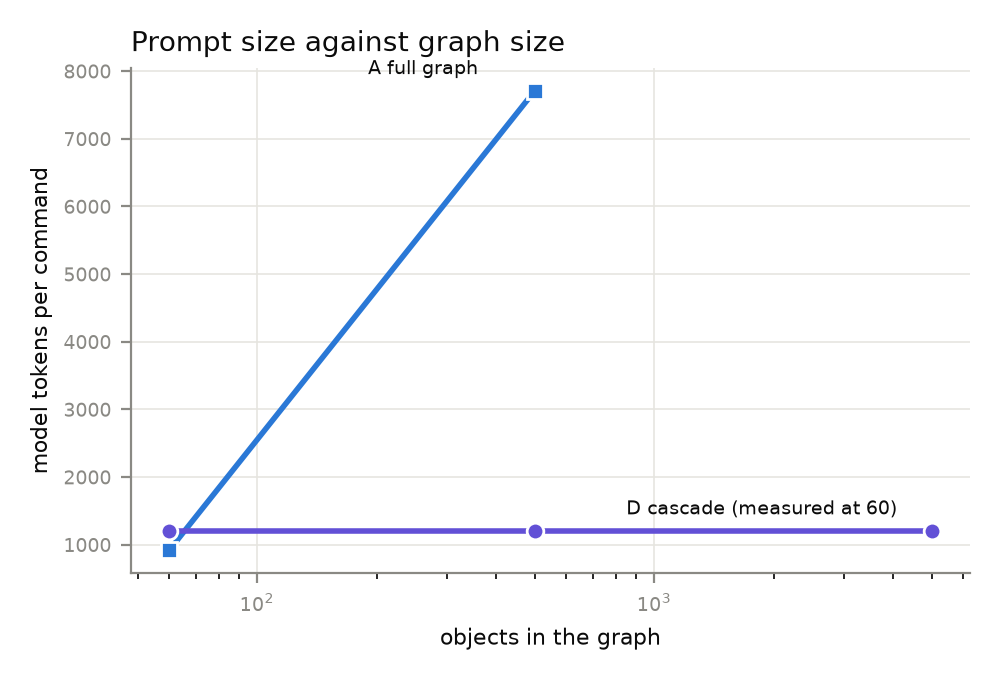
\includegraphics[width=0.92\columnwidth]{figures/tokens_vs_size.png}
\caption{Model tokens per command against graph size. A was not run at 5{,}000 objects: the prompt exceeds the context.}\label{fig:tokens}
\end{figure}

\textbf{Limits.} Coverage is marginal, not per command type; it is capped by the filter: 5 of 114 test commands lose
the right object before ranking, so no $\alpha$ exceeds 95.6\% coverage. At $\alpha\le0.1$ the sets are large
($\approx$38 of $\approx$50 candidates), so the guarantee is informative only from $\alpha\approx0.2$.

\subsection{Q4. Robustness, Scalability and Response Quality}
We compare (A) the full graph in the prompt, (B) CLIP top-1, (C) the VLM always over the CLIP top-5, and (D) our
router ($\alpha{=}0.1$, APS, $s{=}6$ tuned, $K{=}9$). The data are 60 objects photographed from Wikimedia Commons on a
real competition layout (4 rooms, 16 surfaces) and 232 commands of five types, each in English and Spanish,
split by group into 118 calibration and 114 test commands. \emph{Correctness} is accuracy of the returned object;
\emph{completeness} is the share of right objects inside the set (multi-answer commands); \emph{consistency} is
agreement across 5 repeats and between English/Spanish paraphrases. All runs use the same snapshot, crops, model
digests, temperature 0 and seed 0.

\begin{table}[t]
\centering\footnotesize
\caption{Test split, 5 repeats. Tokens include the parse.}\label{tab:main}
\setlength{\tabcolsep}{3pt}
\begin{tabular}{lccccc}
\toprule
Method & Acc. & Tokens & VLM/cmd & p50 (s) & Paraphr. \\
\midrule
A full graph & 70.2\% & 925 & 0 & 0.27 & 86.0\% \\
B CLIP & 78.1\% & 263 & 0 & 0.60 & 87.7\% \\
C VLM always & 77.0\% & 1395 & 0.97 & 2.12 & 86.5\% \\
D router & \textbf{81.4\%} & 1201 & 0.84 & 0.93 & \textbf{89.3\%} \\
\bottomrule
\end{tabular}
\vspace{2pt}

\begin{tabular}{lccccc}
\toprule
Method & attribute & room & spatial & abstract & negation \\
\midrule
A & 73.3 & 78.6 & 57.1 & \textbf{72.2} & 50.0 \\
B & 91.7 & \textbf{85.7} & \textbf{78.6} & 33.3 & 62.5 \\
C & 96.3 & 64.3 & 57.1 & 33.3 & \textbf{87.5} \\
D & \textbf{98.0} & 64.3 & 64.3 & 50.0 & \textbf{87.5} \\
\bottomrule
\end{tabular}
\end{table}

\begin{figure}[t]
\centering
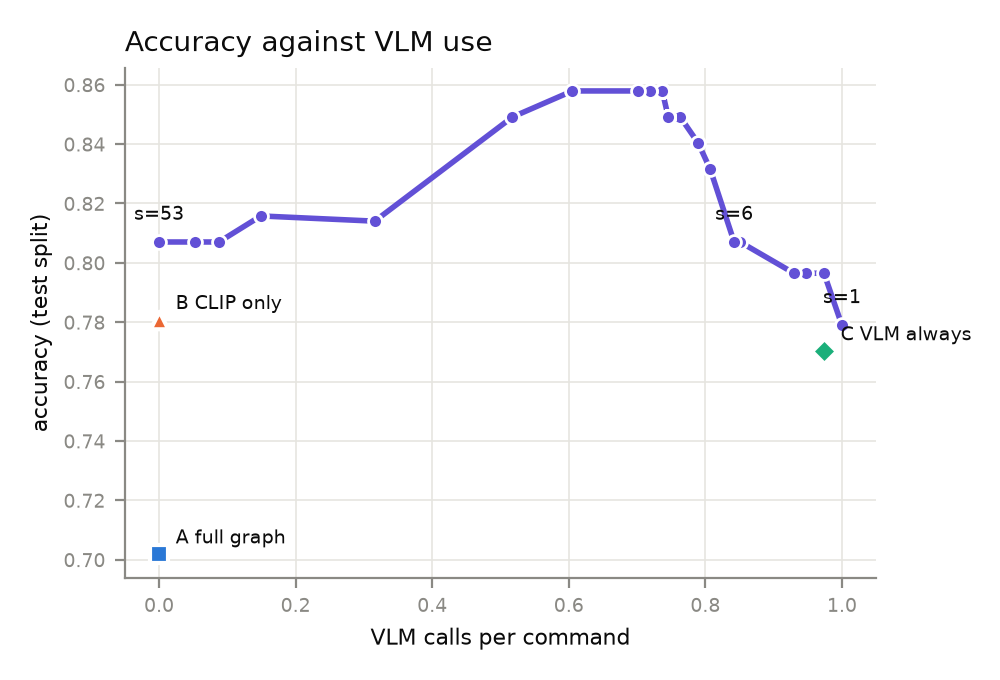
\includegraphics[width=\columnwidth]{figures/routing.png}
\caption{Accuracy against VLM calls when CLIP answers sets up to $s$ (test split).}\label{fig:routing}
\end{figure}

D is the most accurate and the most consistent across languages (Table~\ref{tab:main}); repeat agreement is
$\ge$99.6\% for every method and the parse agreed in 100\% of repeats. The VLM helps on attributes (91.7$\to$98.0\%)
and negation (62.5$\to$87.5\%) but hurts room and spatial commands (85.7$\to$50.0\%,
78.6$\to$50.0\%), where geometry already did the work and crops carry no location. A is best on abstract commands
because it reads labels, not appearance. Figure~\ref{fig:routing} sweeps $s$: escalating everything ($s{=}1$) costs one
VLM call per command for 77.9\%; mid-range $s$ reaches 85.8\% with 0.61--0.74 calls; never escalating gives 80.7\%
at zero VLM cost. The calibration-tuned $s{=}6$ is conservative on test. Lowering the coverage target is the other
knob: at $\alpha{=}0.2$ the APS set shrinks from 5.0 (threshold) to 1.7 candidates and D answers 80.7\% with
273 tokens, CLIP's cost. \textbf{Robustness:} with 25\% of labels swapped within their category, A drops to
59.6\%, B to 70.2\% and D to 77.2\%. \textbf{Scalability:} padding the house to 5{,}000 objects,
\textsc{select} stays at 11\,ms, the brute-force \emph{next to} filter grows to 895\,ms for 200 anchors while the
KD-tree takes 5.5\,ms, and A is no longer runnable.

\subsection{Q5. Limitations and Algorithmic Next Steps}
\textbf{Limitations.} Images are web photos, not robot crops; conformal sets are large at $\alpha\le0.1$;
the VLM lacks location context; 114 test commands give $\pm$4\% binomial error.
\textbf{(1) Type-conditional routing.} Calibrate one threshold per parsed command type (Mondrian conformal) and
never escalate room/spatial commands. Expected: recover the 29--36 points the VLM loses there. Evaluate per-type
coverage and accuracy on the same split.
\textbf{(2) Attention as an error detector.} Offline, the VLM's answer-token attention fell on the right crop in
96.7\% of its correct answers but in only 14.3\% of its wrong ones. Asking when attention and answer disagree
could turn errors into questions. Evaluate error/ask trade-off; attention needs eager kernels, so measure cost on the Orin.
\textbf{(3) Adaptive visual tokens.} Prune grid tokens whose attention mass falls outside the top-$P$ in early
layers (FastV~\cite{chen2024fastv}, AVQ~\cite{vandendool2026avq}). Expected: fewer prefill tokens per call.
Evaluate retained tokens against accuracy and latency.

\section{Part II: Project Report}

\textbf{Overview.} The target is RoboCup@Home's Finals and GPSR tasks, where a robot must find objects it saw
earlier. The repository is a standalone library: a pure core (graph, conformal sets, routing) behind ports for CLIP,
LLM, VLM and clock, with local adapters (Ollama, PyTorch) and ROS 2 adapters for the robot. Resource constraints:
one edge GPU, one model loaded at a time, and a competition clock. Quality requirement: coverage $\ge1-\alpha$ and
accuracy above CLIP alone.

\textbf{M1 --- Core algorithm (implemented).} Parse, geometric filter, fused scoring, split conformal sets
(threshold and APS), calibration and routing are implemented and unit-tested (22 offline tests plus integration
tests against Ollama). Against the unoptimized baseline, D is 11.2 points more accurate than A and its LLM cost
does not grow with the graph (Table~\ref{tab:main}, Section~Q3).

\textbf{M2 --- Deterministic evaluation (implemented).} 232 fixed commands with verifiable answer sets; objective
accuracy, completeness and coverage; 5 repeats; pinned model digests, temperature 0, seed 0 and one loaded model.
Deterministic parts (filter, scoring, sets) are checked to return identical output for an identical parse; LLM and VLM
variability is measured separately (parse agreement 100\%, decision agreement $\ge$99.6\%). The run is checkpointed
and resumable, so results survive crashes without re-sampling.

\textbf{M3 --- Quality preservation and allocation (designed).} Objective: minimize VLM calls per command subject
to accuracy $\ge$ CLIP + 3 points, coverage $\ge 1-\alpha$, and paraphrase agreement $\ge$ 85\%. Allocation knobs
are $\alpha$, $s$ and $K$; we will select them on calibration data only, then report test numbers once.

\textbf{M4 --- Benchmark (planned).} The same pipeline on the Jetson Orin with robot crops from the competition
arena, recording memory, latency and power mode; comparisons against brute force vs.\ KD-tree for spatial queries,
the full-graph prompt, and fixed top-$k$ verification, across graph sizes from 60 to 5{,}000 objects.

\textbf{Repository and roadmap.} Done: core, adapters, 60-object dataset, 232 commands, evaluation, report generator,
offline grounding analysis. Next: (i) type-conditional calibration; (ii) robot crops and ROS 2 integration;
(iii) Orin benchmark; (iv) attention-based abstention and visual token pruning.

\bibliographystyle{IEEEtran}
\bibliography{refs}

\appendix

\subsection{Proof of the Coverage Theorem}
Let $v_{n+1}=\min_{o\in Y}V(o;t)$ for the test command and $k=\lceil(n+1)(1-\alpha)\rceil$. If $k>n$ then
$\hat q=+\infty$, $\cset=C$ and coverage is trivially the filter's. Otherwise, by exchangeability of
$(v_1,\dots,v_{n+1})$, the rank of $v_{n+1}$ is uniform on $\{1,\dots,n+1\}$ (ties broken at random), so
$P(v_{n+1}\le v_{(k)})\ge k/(n+1)\ge1-\alpha$, where $v_{(k)}=\hat q$ is the $k$-th smallest calibration score.
Finally $v_{n+1}\le\hat q$ means some $o\in Y$ has $V(o;t)\le\hat q$, i.e.\ $o\in\cset$. For APS, $V$ is the softmax mass
above $o$, which is monotone in rank, so $\cset$ is a prefix of the ranking and the same argument applies.

\subsection{Extended Results}
\begin{table}[h]
\centering\footnotesize
\caption{Router against $\alpha$ and set construction (test split).}
\setlength{\tabcolsep}{3pt}
\begin{tabular}{llccccc}
\toprule
$\alpha$ & Set & Coverage & Acc. & $|\cset|$ & VLM/cmd & Tokens \\
\midrule
0.05 & threshold & 95.6\% & 82.3\% & 46.1 & 0.85 & 1210 \\
0.05 & APS & 95.6\% & 83.2\% & 46.1 & 0.85 & 1210 \\
0.10 & threshold & 95.6\% & 83.2\% & 39.9 & 0.83 & 1191 \\
0.10 & APS & 95.6\% & 81.4\% & 38.0 & 0.84 & 1201 \\
0.20 & threshold & 88.6\% & 78.8\% & 5.0 & 0.37 & 673 \\
0.20 & APS & 87.7\% & 80.7\% & 1.7 & 0.01 & 273 \\
\bottomrule
\end{tabular}
\end{table}

\begin{table}[h]
\centering\footnotesize
\caption{Scaling by padding the house with near-copies of its objects.}
\setlength{\tabcolsep}{3pt}
\begin{tabular}{lcccc}
\toprule
Objects & A tokens & \textsc{select} (ms) & \emph{next to} brute (ms) & KD-tree (ms) \\
\midrule
60 & 913 & 8.4 & 12.6 & 9.8 \\
500 & 7{,}708 & 4.0 & 98.2 & 6.7 \\
5{,}000 & -- & 11.0 & 895.0 & 5.5 \\
\bottomrule
\end{tabular}
\end{table}

\textbf{Grounding (offline).} Qwen2.5-VL-7B in Hugging Face (4-bit, eager attention) over the same grids, on the
114 test commands (104 with a right crop shown): answer accuracy 86.5\%, the answer token's attention peaks on a
right crop in 85.6\% of cases and on the chosen crop in 90.4\%; attention fails to point at the right crop when the
answer is wrong (14.3\% against 96.7\%), a known caveat of reading attention as explanation~\cite{jain2019attention}.

\begin{figure}[h]
\centering
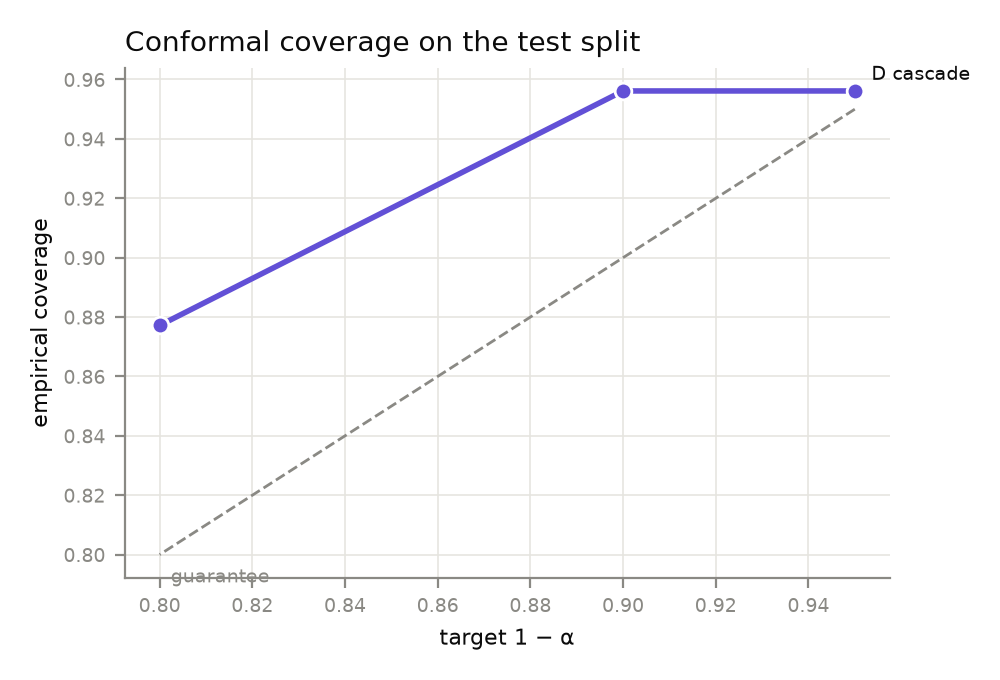
\includegraphics[width=0.9\columnwidth]{figures/coverage.png}
\caption{Empirical coverage of the APS set against the target $1-\alpha$.}
\end{figure}

\textbf{Reproduction.} Raw records, per-host tables and figures are written to \texttt{results/}.
\begin{flushleft}\footnotesize
\texttt{pip install -r requirements.txt}\\
Ollama with \texttt{OLLAMA\_MAX\_LOADED\_MODELS=1};\\
pull \texttt{qwen3:8b} and \texttt{qwen2.5vl:7b}\\
\texttt{python scripts/embed\_images.py}\\
\texttt{python -m eval.run}\\
\texttt{python -m eval.report}\\
\texttt{python -m eval.grounding}
\end{flushleft}

\end{document}
